\chapter{Multipath TCP}
\label{chap:multipathtcp}

\section{Transmission Control Protocol (TCP)}
MPTCP is an extension of regular TCP, the ubiquitous protocol for highly reliable host-to-host communication in a packet-switched computer network. A proper introduction of the fundamental of TCP is due.


The reasons why TCP became a de-facto standard in modern computer communication has been briefly mentioned in the introductory part of the paper. A more technical analysis shows that TCP maintains good levels of reliability for the connection independently from the lower layers it depends on for the raw transmission of bits. TCP is indeed able to handle possible data loss, data damaging, data duplication, out of order delivery of data. In order to do this, the data to be transmitted is split into a sequence of TCP packets, each containing an additional \textit{TCP header} with the information needed to operate the protocol functionalities. Such functionalities are [\href{https://tools.ietf.org/html/rfc793}{ref}]:

\begin{itemize}
  \item \textit{Basic Data Transfer}: sending continuous stream of octets in each direction between its users, identified by the 4-tuple: source IP address, source port, destination IP address, destination port. The IP address allows to route packets to the destination machines, while the port values direct the content of the packet to the right application within a host;
  \item \textit{Reliability}: in-order, reliable data transfer is achieved by adding a sequence number to each transmitted octet and using ACK signals and timeouts to possibly trigger retransmission of lost packets. TCP assures that no transmission errors will affect the delivery of the data assuming that the network will not be completely partitioned;
  \item \textit{Flow Control}: the receiver can control the amount of data sent by the sender returning a "window" value, so that it is possible to avoid buffer congestion;
  \item \textit{Multiplexing}: a single host is allowed to use multiple independent TCP connections simultaneously thanks to the port value available in the protocol. This value, together with the host address assigned at the internet communication layer, forms a socket, that is the actual endpoint of a TCP connection;
  \item \textit{Connections}: TCP initializes and maintains status information regarding each connection and the data stream between a pair of sockets in order to provide all its functionalities. Such status information is initialized during a first handshake procedure, and released only upon connection termination;
  \item \textit{Precedence and Security}: such aspects of the TCP connections can be tuned by users, but default values are provided.
\end{itemize}

As noted above, all these features are made possible by processing the bits at the TCP header. Such structured set of information is mostly static and predefined, so that at each position in the header corresponds a well known portion of the TCP data. The TCP header looks like the one in Figure \ref{fig:tcp_header}.

\begin{figure}[!htb]
\centering
\includegraphics[width=0.75\textwidth]{images/tcp_header}
\caption{The TCP header format}
\label{fig:tcp_header}
\end{figure}

The \textit{Source Port} and \textit{Destination Port}, together with the source and destination IP addresses provided in the upper IP header (not shown in figure \ref{fig:tcp_header}), are the means for identifying the two endpoints of the TCP connection. \textbf{These static fields clearly shows the single-path fundamental design of the protocol}. \textit{Sequence Number}, \textit{Acknowledgment Number} and \textit{Data Offset} are three fields used to guarantee reliable and in-order data transmission; numbering each octet it is possible to put them in sequence and acknowledge them in a cumulative way, so that by acknowledging sequence number X means that all packets up to but not including X has been received. This system, together with timeouts, allows for retransmission of lost packets.
Other interesting fields in the header are: the \textit{Window} field, which allows to achieve congestion control by telling to the sender the range of sequence numbers the data receiver is prepared to accept in a particular instance of time; the \textit{Checksum} field, which guarantees that data has not been modified on its way to the destination (thus being part of the reliability aspect of the protocol).


A component of the TCP header that is fundamental for MPTCP is the \textit{Options} field, which was firstly introduced as a free space for future additions to the protocol. In this specific case, the TLV solution is adopted to process the data inside the field. "TLV" stands for \textit{type-length-value}, where the type is the ID value uniquely identifying the option, the length is the number of bytes of the option, whereas the value represents the actual option content. This particular design allows to skip unknown options at the receiver by simply checking the length value and moving the pointer accordingly. An important limitation for this field is that its total length cannot be higher than 40 bytes [ref].

\section{MPTCP Design}
MPTCP functional goals are to increase resilience of the connectivity and efficiency of the resource usage.
Such goals can be found very similar in other multipathing solutions as the ones described in section [add section], but what is really unique about MPTCP protocol design is the set of its compatibilities goals [\href{https://tools.ietf.org/html/rfc6182}{ref}]:

\begin{itemize}
  \item \textit{Application compatibility} aims at instantiating a protocol that can be fully operational with no modifications for the applications using it. This means that the networking APIs and the overall service model of regular TCP has to be maintained with MPTCP; the entire MPTCP functioning is handled transparently by the underlying system. Such transparency must be maintained also in terms of throughput, resilience and security for the connection, that cannot be deteriorated with respect to the current TCP standards;
  \item \textit{Network compatibility} is a similar goal for MPTCP, which is supposed to work out of the box with the current underlying network layer and the ones below it. The main reason still resides in the possibility of achieving a smooth wide-spread deployment of the protocol on the current infrastructure;
  \item \textit{Users compatibility} is a corollary to both network and application compatibility, which states that MPTCP flows must be fair to regular TCP connection in case of shard bottlenecks.
\end{itemize}


All these compatibilities requirements should explain the very fundamental decision of developing the new multipath protocol at the transport layer, and more specifically as an extension of regular TCP. Let's take into consideration the traditional TCP protocol stack and compare it to the new MPTCP stack in figure \ref{fig:stack}.

\begin{figure}[!htb]
\centering
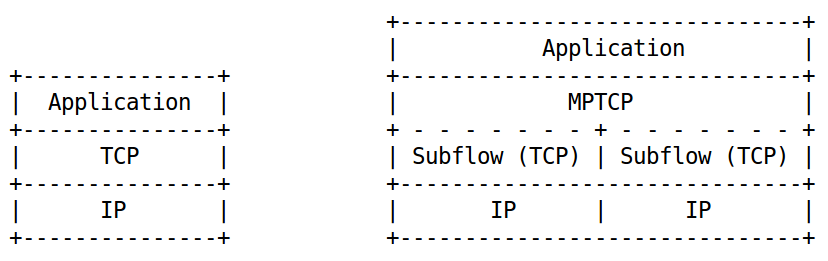
\includegraphics[width=0.75\textwidth]{images/stack}
\caption{The TCP and MPTCP protocol stacks}
\label{fig:stack}
\end{figure}

To achieve the required compatibility goals, changes had to be applied to layers lower than the application layer, so that current programs do not have to be upgraded to make use of multipath; on the other side, the new protocol had to be placed at layers above the network layer, which is the last layer still operating at the networking infrastructure before the transport layer, the latter being the first layer operating at the end systems. The choice of working at the transport layer was indeed the only available option. Within that option, the choice of maintaining TCP as the fundamental operating protocol for MPTCP was still required for similar compatibility reasons; for this very purpose engineers decided to add all the required options for MPTCP functioning inside the TCP Option field in the TCP header. In this way, MPTCP-aware systems can process the MPTCP options for multipathing, but if a system that is not MPTCP-aware receives a MPTCP connection-request, it would simply discard the MPTCP options and threat such message as a plain TCP connection-request. For what regards applications, they don't need to be changed either since MPTCP would be inserted into the network stack at the operating system level; it would automatically split the data buffered from the application layer and send it through different subflows, according to the number of available endpoints at the connected hosts.

\vspace{5mm}
There is only a single generic MPTCP option, to which has been assigned the value 30 as the "Kind" identifier. At a lower level it is possible to identify a set of eight MPTCP option subtypes:

\begin{itemize}
  \item MP\_CAPABLE (Multipath Capable);
  \item MP\_JOIN (Join Connection);
  \item DSS (Data Sequence Signal);
  \item ADD\_ADDR (Add Address);
  \item REMOVE\_ADDR (Remove Address);
  \item MP\_PRIO (Change Subflow Priority);
  \item MP\_FAIL (Fallback);
  \item MP\_FASTCLOSE (Fast Close).
\end{itemize}

All of these options are used to handle the multiple subflow in a MPTCP session and the data transfer within the same session, thus falling into two main categories: control plane and data plane. 

\subsection{Control Plane}
All the MPTCP options used to manage MPTCP sessions are reported and explained here, including all the details on how to set a new session and add/remove subflows.

\subsection{Data Plane}
This part concerns all the MPTCP options used to manage the data flow in a MPTCP session, including how the byte stream is subdivided into different subflow and how the original order of the packets is provided at the receiver.

\section{MPTCP Deployment}
After having explained all the technicalities about the protocol, it is now possible to talk about its deployment status and the problems encountered by pairing MPTCP with current infrastructures. This might seem a bit outside the scope of the thesis, but it is worth mentioning that the \textit{deployment status} and \textit{implementations} are a good indicator of how much MPTCP is important in the Internet community and they are good topics to motivate the thesis work. Also \textit{middleboxes compatibility} is indeed a fundamental part of the MPTCP security evaluation, being monitoring and detection equipment part of these middleboxes.

\subsection{Middleboxes Compatibility}
This section will be quite technical and it is supposed to list the most important middle-boxes and their impact/effect on a MPTCP connection. These boxes include NATs, proxies and firewalls. This part should clearly state why MPTCP widespread adoption is a big challenge.

\subsection{Implementations}
Despite the previously described problematics, MPTCP is a big bet in the IETF community and many implementations have been developed for the most common OSes, listed in this section (with some history notions).

\subsection{Deployment Status}
It should be interesting for the reader to go through some examples of real world's scenarios in which MPTCP is used successfully. Here it is possible to cite some important achievements related to MPTCP (for example the highest throughput ever reached with the new protocol).
If available, it would be also good to show some graphs about MPTCP adoption rate or similar.